\chapter{Project Planning Schedule}
\makeatletter\@mkboth{}{Appendix}\makeatother

\begin{table}[!ht]
    \mytable
    \caption{Project goals and planned time frame.}
    \begin{tabularx}{\linewidth}{@{} c  X @{}}
        \toprule
        Time Frame / Date  & \multicolumn{1}{c}{Goal} \\
        \midrule
        12 - 29 June 2018 & Initial research and development of software on existing feature extraction techniques. Set up project outline. \\
        \midrule
        3 - 20 July 2018 & Research and development of TensorFlow and CNN models. \\
        \midrule
        24 July - 5 August 2018 & Initial identification and phrasing of problem and proposed solution. Write abstract. \\
        \midrule
        6 August 2018 & Submit first draft of abstract. \\
        \midrule
        6 - 12 August 2018 & Research Google Cloud Platform and available services. \\
        \midrule
        13 - 31 August 2018 & Develop and test feature extraction software run on Datalab. \\
        \midrule
        17 - 30 September 2018 & Extract features from speech data on Google Datalab. Write initial literature study. Develop and test feature evaluation software. \\
        \midrule
        30 September - 7 October 2018 & Develop high-throughput computing technique for feature evaluation using GCP. Finish literature study on feature extraction and evaluation. \\
        \midrule
        8 October 2018 & Submit first initial report draft. \\
        \midrule
        8 - 21 October 2018 & Run feature evaluation experiments using GCP technique. Ensure software is working correctly and fix any errors. Write experimental setup chapter. \\
        \midrule
        22 - 29 October 2018 & Run any remaining experiments. Finish writing first full draft of report. \\
        \midrule
        30 October 2018 & Submit final draft. \\
        \midrule
        30 October - 4 November 2018 & Amend report and finish any remaining work. Clean up code base. \\
        \midrule
        5 November 2018 & Submit report. \\
        \bottomrule
    \end{tabularx}
    \label{tbl:schedule}
\end{table}

\chapter{Outcomes Compliance}
\makeatletter\@mkboth{}{Appendix}\makeatother

\newcolumntype{R}[1]{>{\centering\let\newline\\\arraybackslash\hspace{0pt}}m{#1}}
\begin{table}[h]
    \mytable
    \caption{The ECSA exit level outcomes and how they were achieved.}
    \begin{tabularx}{\linewidth}{@{} R{4cm} X R{1.3cm} @{}}
        \toprule
        Outcomes & Outcome Description & Pages \\ 
        \midrule
        \textbf{ELO 1: Problem Solving} & The problem of processing all required tasks within a reasonable time was identified and analysed. Various solutions were researched and tested until a suitable solution (GCP services) was identified and implemented. & \textbf{16-18} \\
        \midrule
        \textbf{ELO 2: Application of scientific and engineering knowledge} & Understanding and applying the concepts of spectrograms, filterbanks, MFCCs and convolution required knowledge of mathematics, advanced frequency and cepstral analysis. Skills in computer science and machine learning were necessary for the application and manipulation of CNNs. & \textbf{5-9, 17-18} \\
        \midrule
        \textbf{ELO 3: Engineering Design} & The high-throughput feature evaluation software architecture was designed, developed, analysed, tested and documented. This architecture was developed to be higly extendable and was communicated clearly, the impact and possible uses described. & \textbf{15-18, 31} \\
        \midrule
        \textbf{ELO 4: Investigations, experiments and data analysis} & Various experiments were conducted to evaluate our models, and we make comparisons with previous work by using consistent evaluation metrics and a benchmark dataset. Results are analysed and conclusions are made. & \textbf{20-26, 29-30} \\
        \midrule
        \textbf{ELO 5: Engineering  methods,  skills  and  tools,  including  Information  Technology} & Software languages such as Python, Cython, Node.js were used. Multiple software frameworks and tools such as Jupyter Notebooks, GCE, GCS, Cloud Functions and Datalab were researched and implemented. & \textbf{12, 15-18} \\
        \midrule
        \textbf{ELO 6: Professional and technical communication} & This technical report makes use of appropriate structure, style, and language, and was developed with \LaTeX. & \textbf{1-31} \\
        \midrule
        \textbf{ELO 8: Individual work} & All research, experiments, software development and report writing was done individually.  & \textbf{9-10, 15-16} \\
        \midrule
        \textbf{ELO 9: Independent Learning Ability} & An understanding and high-level competency in TensorFlow CNNs, GCP services and conducting experiments was obtained completely independently. & \textbf{9-10, 15-16} \\
        \bottomrule
    \end{tabularx}
\label{tbl:elo}
\end{table}

\chapter{First Layer Kernels of VGG16}
\makeatletter\@mkboth{}{Appendix}\makeatother
\label{appen:conv1_1}

\begin{figure}[h]
    \centering
    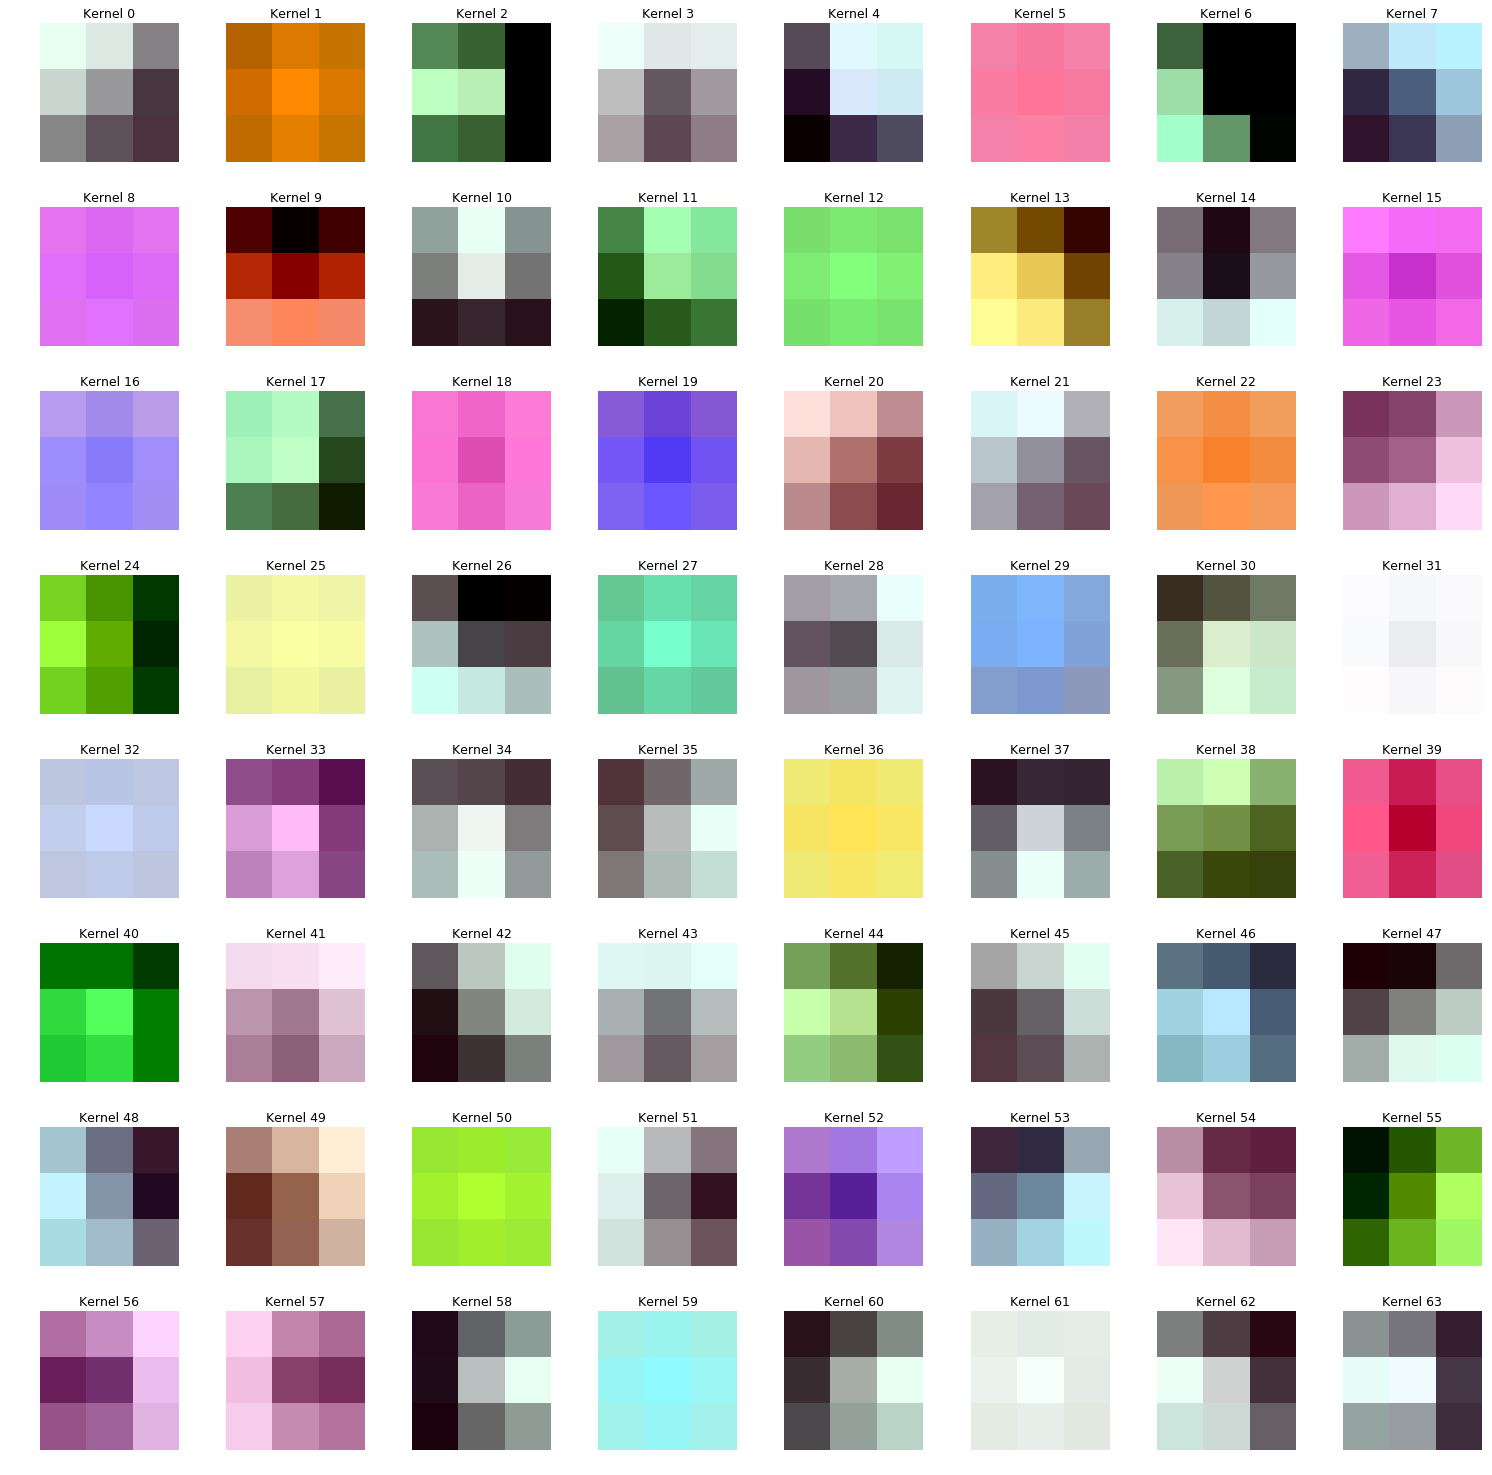
\includegraphics[width=\linewidth]{appendices/fig/conv1_1.png}
    \caption{First layer kernels of VGG16}
    \label{fig:my_label}
\end{figure}

\chapter{Spectrogram features}
\makeatletter\@mkboth{}{Appendix}\makeatother
\label{appen:ap_scores}
\begin{center}
\begin{longtable}{c l l | c l l | c l l }
    \caption{AP scores for the top performing features obtained from spectrograms.}
        \\ \hline
        \# & Feature & AP & \# & Feature & AP & \# & Feature & AP \\ \hline
        1 & \texttt{conv1\_2:27} & $0.186$ & 2 & \texttt{conv2\_1:74} & $0.164$ & 3 & \texttt{conv2\_2:106} & $0.161$ \\
        4 & \texttt{conv2\_2:6} & $0.151$ & 5 & \texttt{conv3\_2:89} & $0.129$ & 6 & \texttt{conv2\_1:119} & $0.120$ \\
        7 & \texttt{conv2\_1:90} & $0.118$ & 8 & \texttt{conv3\_1:119} & $0.115$ & 9 & \texttt{conv1\_2:4} & $0.113$ \\
        10 & \texttt{conv3\_1:251} & $0.111$ & 11 & \texttt{conv1\_1:5} & $0.111$ & 12 & \texttt{conv3\_1:175} & $0.107$ \\
        13 & \texttt{conv3\_1:212} & $0.106$ & 14 & \texttt{conv2\_1:118} & $0.102$ & 15 & \texttt{conv1\_2:52} & $0.095$ \\
        16 & \texttt{conv3\_2:161} & $0.095$ & 17 & \texttt{conv1\_2:2} & $0.092$ & 18 & \texttt{conv3\_2:143} & $0.092$ \\
        19 & \texttt{conv2\_2:64} & $0.091$ & 20 & \texttt{conv3\_3:114} & $0.091$ & 21 & \texttt{conv3\_2:179} & $0.090$ \\
        22 & \texttt{conv1\_1:16} & $0.089$ & 23 & \texttt{conv3\_1:107} & $0.088$ & 24 & \texttt{conv3\_1:57} & $0.087$ \\
        25 & \texttt{conv3\_2:141} & $0.085$ & 26 & \texttt{conv3\_1:247} & $0.084$ & 27 & \texttt{conv2\_1:2} & $0.084$ \\
        28 & \texttt{conv1\_2:25} & $0.083$ & 29 & \texttt{conv2\_2:65} & $0.082$ & 30 & \texttt{conv2\_2:77} & $0.082$ \\
        31 & \texttt{conv3\_1:205} & $0.082$ & 32 & \texttt{conv2\_2:117} & $0.082$ & 33 & \texttt{conv1\_1:31} & $0.077$ \\
        34 & \texttt{conv2\_1:110} & $0.077$ & 35 & \texttt{conv2\_2:90} & $0.076$ & 36 & \texttt{conv2\_2:73} & $0.075$ \\
        37 & \texttt{conv3\_2:50} & $0.074$ & 38 & \texttt{conv1\_2:31} & $0.073$ & 39 & \texttt{conv2\_1:9} & $0.070$ \\
        40 & \texttt{conv2\_1:61} & $0.070$ & 41 & \texttt{conv2\_1:21} & $0.068$ & 42 & \texttt{conv3\_3:88} & $0.065$ \\
        43 & \texttt{conv3\_2:156} & $0.061$ & 44 & \texttt{conv2\_2:127} & $0.061$ & 45 & \texttt{conv2\_2:118} & $0.059$ \\
        46 & \texttt{conv3\_2:35} & $0.059$ & 47 & \texttt{conv2\_1:7} & $0.059$ & 48 & \texttt{conv3\_3:62} & $0.058$ \\
        49 & \texttt{conv2\_2:51} & $0.058$ & 50 & \texttt{conv2\_1:62} & $0.057$ & 51 & \texttt{conv3\_3:249} & $0.057$ \\
        52 & \texttt{conv3\_1:43} & $0.056$ & 53 & \texttt{conv3\_2:129} & $0.056$ & 54 & \texttt{conv2\_1:53} & $0.056$ \\
        55 & \texttt{conv3\_1:38} & $0.055$ & 56 & \texttt{conv2\_1:38} & $0.054$ & 57 & \texttt{conv2\_1:24} & $0.054$ \\
        58 & \texttt{conv3\_2:205} & $0.053$ & 59 & \texttt{conv2\_1:52} & $0.053$ & 60 & \texttt{conv3\_3:125} & $0.052$ \\
        61 & \texttt{conv3\_3:159} & $0.051$ & 62 & \texttt{conv3\_2:109} & $0.051$ & 63 & \texttt{conv2\_1:100} & $0.051$ \\
        64 & \texttt{conv3\_1:201} & $0.050$ & 65 & \texttt{conv3\_1:56} & $0.050$ & 66 & \texttt{conv1\_2:9} & $0.050$ \\
        67 & \texttt{conv2\_1:27} & $0.050$ & 68 & \texttt{conv3\_2:77} & $0.049$ & 69 & \texttt{conv2\_1:50} & $0.049$ \\
        70 & \texttt{conv3\_1:53} & $0.049$ & 71 & \texttt{conv2\_1:5} & $0.049$ & 72 & \texttt{conv3\_1:20} & $0.048$ \\
        73 & \texttt{conv2\_1:71} & $0.048$ & 74 & \texttt{conv2\_2:40} & $0.046$ & 75 & \texttt{conv3\_1:130} & $0.046$ \\
        76 & \texttt{conv3\_1:178} & $0.046$ & 77 & \texttt{conv2\_1:16} & $0.045$ & 78 & \texttt{conv3\_1:27} & $0.043$ \\
        79 & \texttt{conv2\_2:105} & $0.042$ & 80 & \texttt{conv2\_2:94} & $0.042$ & 81 & \texttt{conv2\_1:94} & $0.042$ \\
        82 & \texttt{conv3\_2:37} & $0.042$ & 83 & \texttt{conv1\_2:45} & $0.042$ & 84 & \texttt{conv3\_3:213} & $0.041$ \\
        85 & \texttt{conv2\_1:55} & $0.041$ & 86 & \texttt{conv2\_1:48} & $0.041$ & 87 & \texttt{conv3\_2:63} & $0.040$ \\
        88 & \texttt{conv3\_1:120} & $0.040$ & 89 & \texttt{conv3\_1:16} & $0.040$ & 90 & \texttt{conv2\_1:120} & $0.040$ \\
        91 & \texttt{conv3\_2:255} & $0.040$ & 92 & \texttt{conv3\_1:250} & $0.040$ & 93 & \texttt{conv3\_2:4} & $0.040$ \\
        94 & \texttt{conv1\_2:37} & $0.039$ & 95 & \texttt{conv2\_2:13} & $0.039$ & 96 & \texttt{conv3\_1:198} & $0.039$ \\
        97 & \texttt{conv3\_1:18} & $0.039$ & 98 & \texttt{conv3\_2:216} & $0.039$ & 99 & \texttt{conv3\_2:42} & $0.038$ \\
        100 & \texttt{conv3\_2:31} & $0.038$ & 101 & \texttt{conv2\_1:66} & $0.038$ & 102 & \texttt{conv1\_2:46} & $0.038$ \\
        103 & \texttt{conv3\_2:34} & $0.038$ & 104 & \texttt{conv3\_1:171} & $0.038$ & 105 & \texttt{conv3\_1:245} & $0.037$ \\
        106 & \texttt{conv3\_3:80} & $0.037$ & 107 & \texttt{conv3\_2:210} & $0.036$ & 108 & \texttt{conv2\_2:126} & $0.036$ \\
        109 & \texttt{conv3\_2:187} & $0.035$ & 110 & \texttt{conv3\_3:10} & $0.035$ & 111 & \texttt{conv3\_1:195} & $0.034$ \\
        112 & \texttt{conv3\_1:219} & $0.034$ & 113 & \texttt{conv3\_2:121} & $0.034$ & 114 & \texttt{conv2\_1:73} & $0.034$ \\
        115 & \texttt{conv3\_2:165} & $0.033$ & 116 & \texttt{conv1\_2:34} & $0.033$ & 117 & \texttt{conv3\_1:30} & $0.033$ \\
        118 & \texttt{conv1\_2:13} & $0.033$ & 119 & \texttt{conv2\_1:106} & $0.033$ & 120 & \texttt{conv3\_2:87} & $0.032$ \\
        121 & \texttt{conv3\_2:28} & $0.032$ & 122 & \texttt{conv3\_1:218} & $0.032$ & 123 & \texttt{conv2\_1:96} & $0.032$ \\
        124 & \texttt{conv1\_1:1} & $0.032$ & 125 & \texttt{conv2\_2:4} & $0.031$ & 126 & \texttt{conv3\_3:109} & $0.031$ \\
        127 & \texttt{conv3\_1:72} & $0.031$ & 128 & \texttt{conv3\_2:114} & $0.031$ & 129 & \texttt{conv2\_1:18} & $0.031$ \\
        130 & \texttt{conv2\_1:36} & $0.031$ & 131 & \texttt{conv2\_1:15} & $0.031$ & 132 & \texttt{conv3\_3:234} & $0.030$ \\
        133 & \texttt{conv2\_2:63} & $0.030$ & 134 & \texttt{conv2\_1:49} & $0.030$ & 135 & \texttt{conv3\_1:157} & $0.030$ \\
        136 & \texttt{conv3\_2:48} & $0.030$ & 137 & \texttt{conv3\_2:195} & $0.029$ & 138 & \texttt{conv1\_2:60} & $0.029$ \\
        139 & \texttt{conv1\_2:26} & $0.029$ & 140 & \texttt{conv2\_1:112} & $0.029$ & 141 & \texttt{conv3\_2:153} & $0.028$ \\
        142 & \texttt{conv3\_2:144} & $0.028$ & 143 & \texttt{conv3\_2:5} & $0.028$ & 144 & \texttt{conv3\_2:196} & $0.028$ \\
        145 & \texttt{conv3\_2:167} & $0.028$ & 146 & \texttt{conv3\_3:162} & $0.028$ & 147 & \texttt{conv2\_2:11} & $0.027$ \\
        148 & \texttt{conv3\_2:94} & $0.027$ & 149 & \texttt{conv3\_1:172} & $0.027$ & 150 & \texttt{conv1\_2:53} & $0.027$ \\
        151 & \texttt{conv2\_2:102} & $0.026$ & 152 & \texttt{conv1\_2:17} & $0.026$ & 153 & \texttt{conv3\_2:68} & $0.026$ \\
        154 & \texttt{conv2\_2:7} & $0.026$ & 155 & \texttt{conv3\_2:46} & $0.025$ & 156 & \texttt{conv2\_1:35} & $0.025$ \\
        157 & \texttt{conv3\_2:227} & $0.025$ & 158 & \texttt{conv3\_2:39} & $0.025$ & 159 & \texttt{conv3\_3:178} & $0.025$ \\
        160 & \texttt{conv3\_2:140} & $0.025$ & 161 & \texttt{conv3\_2:248} & $0.025$ & 162 & \texttt{conv3\_1:246} & $0.025$ \\
        163 & \texttt{conv1\_1:36} & $0.025$ & 164 & \texttt{conv3\_2:240} & $0.024$ & 165 & \texttt{conv3\_2:208} & $0.024$ \\
        \hline
    \label{tbl:spectrograms_full}
\end{longtable}
\end{center}